%%%%%%%%%%%%%%%%%%%%%%%%%%%%%%%%%%%%%%%%%%%%%%%%%%%%%%%%%%%%%%%%%%%%%%%%%%%%%%%%
%2345678901234567890123456789012345678901234567890123456789012345678901234567890
%        1         2         3         4         5         6         7         8

\documentclass[letterpaper, 10 pt, conference]{ieeeconf}  % Comment this line out
                                                          % if you need a4paper
%\documentclass[a4paper, 10pt, conference]{ieeeconf}      % Use this line for a4
                                                          % paper

\IEEEoverridecommandlockouts                              % This command is only
                                                          % needed if you want to
                                                          % use the \thanks command
\overrideIEEEmargins
% See the \addtolength command later in the file to balance the column lengths
% on the last page of the document



% The following packages can be found on http:\\www.ctan.org
\usepackage{graphics} % for pdf, bitmapped graphics files
\usepackage{epsfig} % for postscript graphics files
%\usepackage{mathptmx} % assumes new font selection scheme installed
%\usepackage{times} % assumes new font selection scheme installed
\usepackage{amsmath} % assumes amsmath package installed
\usepackage{amssymb}  % assumes amsmath package installed

\usepackage{url}
\usepackage[ruled, vlined, linesnumbered]{algorithm2e}
%\usepackage{algorithm}
\usepackage{verbatim} 
%\usepackage[noend]{algpseudocode}
\usepackage{soul, color}
\usepackage{lmodern}
\usepackage{fancyhdr}
\usepackage[utf8]{inputenc}
\usepackage{fourier} 
\usepackage{array}
\usepackage{makecell}
\usepackage{hyperref}

\SetNlSty{large}{}{:}

\renewcommand\theadalign{bc}
\renewcommand\theadfont{\bfseries}
\renewcommand\theadgape{\Gape[4pt]}
\renewcommand\cellgape{\Gape[4pt]}

\newcommand{\rework}[1]{\todo[color=yellow,inline]{#1}}

\makeatletter
\newcommand{\rom}[1]{\romannumeral #1}
\newcommand{\Rom}[1]{\expandafter\@slowromancap\romannumeral #1@}
\makeatother

\pagestyle{plain} 

\title{\LARGE \bf
The approaching to Hand Gesture Recognition, Vehicle Color Recognition, and Handwritten digit recognition
}

\author{ \parbox{3 in}{\centering \bf Ulugbek Shernazarov - U1910253
        % \thanks{*Use the $\backslash$thanks command to put information here}
        \\ Multimedia Application\\
        Inha University in Tashkent\\
        {\tt\small u.shernazarov@student.inha.uz}}
        \hspace*{ 0.5 in}
        \parbox{3 in}{ \centering \bf Prof. Uddin Ahmed Minhaz
        % \thanks{**The footnote marks may be inserted manually}\\
        \\ Multimedia Application\\
        Inha University in Tashkent \\
        {\tt\small 	minhaz.ahmed@gmail.com}}
}

% \author{\bf Ulugbek Shernazarov - U1910253% <-this % stops a space 
% \\ Multimedia Application \\
% Inha University in Tashkent \\
% {\tt\small usernazarov@gmail.com} \\ \\
% Prof. Uddin Ahmed Minhaz%
% \\ Inha University in Tashkent \\
% g}


\begin{document}



\maketitle
\thispagestyle{plain}
\pagestyle{plain}



%%%%%%%%%%%%%%%%%%%%%%%%%%%%%%%%%%%%%%%%%%%%%%%%%%%%%%%%%%%%%%%%%%%%%%%%%%%%%%%%
\section{\bf ABSTRACT}

This project paper intends to take use of effective methods for solving the {\bf Hand Gesture Recognition}, {\bf Vehicle Color Recognition}, and {\bf Handwritten digit recognition}. The gesture recognition, after years of research, remains a difficult subject for the following reasons: outcomes of unclear recognition, unstable systems, and inaccurate recognition. Same for Vehicle Color Recognition: include incorrect olygon identification, insufficient pixel count for estimate in half-circles, and insufficient color contrast for segmentation in the movement. Naturally, Handwritten numbers identification yielded the best results, but I wish to continue researching this to find a better method. In this paper, we will just try to apply all the ideas and approaches we have learned throughout the course in an effort to find the most effective answer to each challenge. As a data foundation, i.e. data sets, the publicly available collection from {\bf kaggle} is regarded.\\

%%%%%%%%%%%%%%%%%%%%%%%%%%%%%%%%%%%%%%%%%%%%%%%%%%%%%%%%%%%%%%%%%%%%%%%%%%%%%%%%
\section{\bf INTRODUCTION}

\subsubsection*{\bf HGR (Hand Gesture Recognition)}

One of the most expressive, typical, and natural types of body language for expressing attitudes and emotions in interpersonal encounters is the Hand Gesture. It is one of the most fundamental issues in computer vision and pattern recognition and has many applications, including virtual reality systems, interactive gaming environments, the ability to recognize sign language, allowing very young children to interact with computers, controlling robots, practicing conducting music, controlling television, controlling automobile interfaces, aiding in learning and teaching, and hand gesture generation. \par

Although there has been substantial development in hand gesture detection, certain major issues, such as rapid and robust, remain difficult to solve. Prior work often emphasizes utilizing whole data series, which invariably contain duplicate information and cause performance degradation. All of these initiatives aim to lessen the computational load on each individual frame, but ignoring all processing plans across all frames would result in a greater computational load than a small number of representative frames, which is a key strategy for significantly reducing computational load. This section of the research is focused on bridging the gap between quick and reliable hand gesture detection utilizing just one common cue, such as RGB, which offers enormous potential in practical usage. \par

\subsubsection*{\bf VCR (Vehicle Color Recognition)}
A system called an Intelligent Transport System (ITS) controls everything related to transportation, from traffic control to law enforcement. Vehicles and their characteristics, such as kind, color, and license plate, are an essential item that ITS has extensively studied. The color of a vehicle is a crucial characteristic for identifying it and offers visual indicators for quick action law enforcement. Identifying a vehicle's color is a particularly difficult task because of a number of elements, including as the weather, the video/image collecting process, and the vehicle's strip configuration. \par

In this study, we offer a convolutional neural network (CNN) technique for recognizing the color of a car. CNNs are a sort of neural network, however they extract characteristics from input using a layer called a convolution layer rather than a fully connected layer. The training mechanism uses stochastic gradient descent as the training method and is quite similar to a typical neural network. \par

\subsubsection*{\bf HDR (Handwritten Digit Recognition)}

Handwritten digit recognition is the process to provide the ability to machines to recognize human handwritten digits. It is a subset of OCR (Object Character Recognition). OCR is a tool that turns written or printed letters into text that has been encoded. For a computer, a picture is simply a collection of pixels, which are nothing more than a list of mixes of values ranging from 0 to 255, such as RGB, B.W., greyscale, etc. A human brain can readily analyze and extract data from a complex image. Pixel values can be used to extract information from a picture. \par
CNN (Convolution Neural Networks) performs better for the HDR. Convolution, as it sounds, is the technique of applying different filters on photographs to bring out their features. Consider an input greyscale picture of size 28x28. The input layer has 784 neurons, each of which has a weight known as activation and a value of grey level matching to the pixels in the input image. In this study, we design a convolution neural network architecture using the MNIST dataset to train the network and predict a real-world handwritten digit using relu (rectified linear unit) and sigmoid activation functions. \par

\section{FLOW GRAPH}

The flow graph is based on HDR, but it is appliable to every instance in our research (we have a set of methods for every study; the only variations would be the characteristics and functions/techniques employed).

\begin{figure}[thpb]
      \centering
      \framebox{\parbox{2.2in}{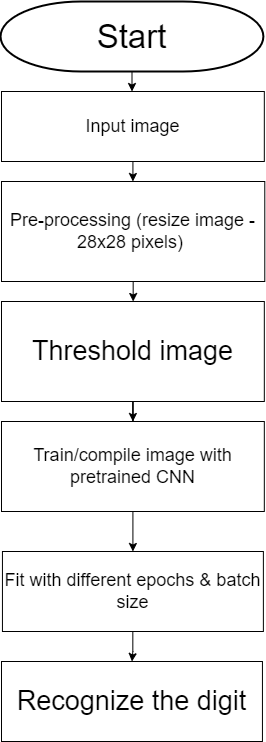
\includegraphics[height=4in, width=2.2in]{Images/dia.png}}}
      \caption{General flow graph approach to each problem}
      \label{fig:1}
\end{figure}

\section{Methodology}
\subsection*{\bf HGR (Hand Gesture Recognition)}
\subsubsection*{\bf Image Entropy} Entropy is a good approach to illustrate the impurity or unpredictability of a set of data since it depends on the environment in which the measurement is made. The distribution of color and intensity in grayscale for a single video frame is shown as $p = {p_1, p_2, ..., p_n}$. For the image frames $x_i$, their image entropy: 
$$E(x_i) = - \sum_{j}p_{x_i}(j)\log_{p_{x_i}}(j)$$
where $p_{x_i}(j)$ denotes the probability density function of image $x_i$.

\subsubsection*{\bf Preprocessing}
For the project base, we will use the dataset available in \href{https://www.kaggle.com/gti-upm/leapgestrecog/version/1}{Hand Gesture Recognition Database}, which contains 20000 images with different hands and hand gestures. There is a total of 10 hand gestures of 10 different people presented in the dataset. There are 5 female subjects and 5 male subjects. The images were captured using the Leap Motion hand tracking device. \par

After downloading and loading all the images into an array that we will call X and all the labels into another array called y, we will split our data into a training set and a test set. We will construct our model using the training set. The test data will next be utilized to determine whether or not our forecasts were accurate. To mimic the unpredictability of our findings, a random state seed is employed. To reduce training loss, the program will shuffle the photos it uses. \par

\subsubsection*{\bf Network Architecture}
The most advanced model architecture for image classification tasks right now is convolutional neural networks (CNNs). Therefore, Our convolutional neural network is made up of many layers with various purposes: the number of filters that the convolutional layer will learn is the initial requirement made by the Conv2D layer. While layers deeper in the network will learn more filters, layers earlier in the network design will learn less convolutional filters. This enables lossless information transfer throughout the network. These filters mimic feature extraction techniques like edge detectors, blob detectors, and others. The values of the filters must be adjusted, although it is customary to utilize powers of 2, starting with 32, 64, and 128 and going up to 256, 512, and 1024. \par

The Conv2D layer also needs the kernel size argument, a 2-tuple that specifies the width and height of the 2D convolution window. The kernel size must be an odd integer, with typical values of 1, 3, 5, and 7. \par

The output volume's spatial dimensions are then minimized by means of MaxPooling2D. Assumptions may be made about the characteristics present in the sub-regions binned, and processing time is decreased. We can observe in this network that while the number of filters we have learnt is growing, the spatial volume of our output is shrinking. \par

The last sort of activation function is known as ReLU, or rectified linear unit. In neural networks, particularly in CNNs, ReLU is the most often employed activation function. ReLU is 0 for all negative values and linear (identity) for all positive values. Because there isn't any challenging arithmetic involved, computation costs are low. Thus, training or running the model may be sped up. Additionally, it converges more quickly due to the application of non-linearities to the model, eliminating the vanishing gradient problem that other activation functions like sigmoid or tanh suffer from. \par

Multiple, fixed-length, 1D sequences $(s_1, s_2,..., s_c)$, where $c \in N$ is the number of sequences, make up the inputs to our network (channels). Three parallel branches each get a direct feed of one of these sequences. In this study, the first branch1, which is incorrectly referred to as the residual branch, is virtually an identity function. In order to lower the danger of overfitting, we pool the input rather than output the model precisely as it was entered. The architecture for feature extraction shared by the second and third branches is described here. \par

The input is handled in the following ways in these two branches. A convolution layer receives the input, while a pooling layer subsamples the output of the convolution layer. Two additional instances of this technique are performed. The number of feature maps employed determines which of the three convolutions are used for a single branch, while the size of the convolution kernels determines which two branches. The temporal convolution layers' two kernel sizes enable the network to operate directly at various time resolutions.\par

The three branches' outputs are combined into a single vector for a single channel. The classifier is a multi layer perceptron that "merges" the concatenated vectors of all the channels. There are the same number of MLP outputs as there are gesture classes. \par

In our tests, we have two branches (high resolution and low resolution branches): J1; 2K, 3 convolution layers, and K (l,) = 8 feature maps for l = 1 or l = 2 and K (l,) = 4 feature maps for l = 3. One hidden layer with 1996 hidden units makes up the multilayer perceptron. Except for the output neurons, which use the softmax activation function, every neuron in our network uses the ReLU activation function: $(x) = ReLU(x) = max(0,x)$. The average pooling method is used by all three subsampling layers, with a temporal pool size of 2. \par

Max pooling takes the maximum value from the features in the neighborhood, whereas average pooling computes the average value of features in a neighborhood (of two time steps in our example). Max pooling performs better than average pooling in image recognition issues, according to empirical evidence. However, our testing on the best pooling approach for this model did not support this conclusion (we see a 0.88\% loss in validation accuracy for the model with maximal pooling as opposed to the average one for the model configuration provided in this study). \par

\subsection*{\bf VCR (Vehicle Color Recognition)}
\subsubsection*{\bf Network Architecture}
Our CNN design consists of two base networks, each with eight levels, for a total of sixteen layers. Our CNN design has a convolutional layer in the top two layers, which performs convolution before normalization and pooling. A layer that performs the same convolutional operation as the convolution process in an image processing technique is known as a convolutional layer. For $I_i$ input image and convolution kernel $k$, the output image:
$$I_o[m,n] = \sum_{j=-\infty}^{\infty} \sum_{i=-\infty}^{\infty} I_i[i,j]\cdot k[m,n]$$
with [m, n] is pixel value at coordinate (m, n). Training process of CNN will learn k, called as kernel, as parameters of convolutional layer. \par

We employ the ReLU activation function in our CNN networks for all levels, even the fully linked layers. Normalization is accomplished using $\alpha = 10^{-4}$, $\beta = 0.75$, and $n=5$:
$$l^i_{x,y} = \frac{k^i_{x,y}}{\big(1+\frac{\alpha}{n} \sum^{i+n/2}_{j=i-n/2} (k^i_{x,y})^2\big)^{\beta}}$$
is the output of the layer activation function for convolution at coordinate $k^i_{x,y}$, where $l^i_{x,y}$ is the normalization result. The pooling procedure comes in at the end of the first two levels. The two types of pooling are mean pooling and maximum pooling. Max pooling will extract the maximum response from the convolutional process, which is a shape with sharp edges, while mean pooling will extract the average of the convolutional process, which is a shape that summarizes the neighborhood. In our architecture, we utilize max pooling with size 3x3 and stride 2. The several layers are divided into two groups, each of which is separate from the others. Although there is no pooling or normalizing procedure, the third and fourth layers are both convolutional layers. Due to the usage of a 3x3 kernel with a pad 1 addition for each boundary, the third and fourth layer outputs are identical to the input. Convolutional layer with just pooling and no normalizing makes up the final layer. \par
The pooling output of the fifth layer from two base networks is concatenated and flattened into a single long vector before moving into a fully-connected layer. The dropout regularization approach was used on the fully linked sixth and seventh layers to reduce overfitting. The output of the network is using {\bf softmax} activation functions, which is defined as the following equation:
$$p(y^{(i)} = j|x^{(i)}; \theta) = \frac{e^{\theta^{T}_j x(i)}}{\sum^k_{l=1} e^{\theta^T_l x^{(i)}}}$$
with $p(y^{(i)} = j|x^{(i)}; \theta)$ is probability of $y^{(i)}$ being class $j$ given input $x^{(i)}$ with weight parameter $\theta$. \par \par
Our CNN design is composed on two base networks with eight layers each for a total of sixteen levels. The first layer uses a total of 48 kernels. The second layer uses a total of 128 kernels. The third layer uses a total of 192 kernels. First, second, and fifth layers all use the pooling technique with the same parameters—a 3x3 pool with a 2-pixel stride. Each 4096-4096-8 neuron in the sixth, seventh, and eighth layers is completely linked, and the dropout regularization approach is used in the sixth and seventh layers. The input to the network is a three channel picture with a resolution of 227x227 and 150,228 dimensions. There are 658,280 neurons altogether that are participating in the networks. \par

With 115 instances per batch, momentum of 0.9, and weight decay of 0.0005, our models were trained using stochastic gradient descent. We make use of Chen dataset for the tests. There are 15601 images of vehicles in the collection, divided into 8 categories according to their color: black, blue, cyan, gray, green, red, white, and yellow. The majority of the class examples are utilized during training. Each illustration is scaled down to 256x256 resolution in a particular color scheme. The four color spaces we employ are RGB, CIE Lab, CIE XYZ, and HSV. Prior to being processed for training, the data was cropped to 227x227 and the training data's mean image was removed. To improve classifier accuracy, data were randomly duplicated during the training phase. We employ a learning rate of 0.01 and constantly reduce by a factor of 10 at multiples of 50,000 with a maximum of 200,000 iterations. \par

SGD, or stochastic gradient descent, is an optimization technique that seeks to determine the least or maximum value of a function. All functions with a gradient or first derivative can be used with SGB. Typically, the system updates the weight parameters while using SGD to minimize the error or loss function. \par

\begin{figure}[thpb]
      \centering
      \framebox{\parbox{2.6in}{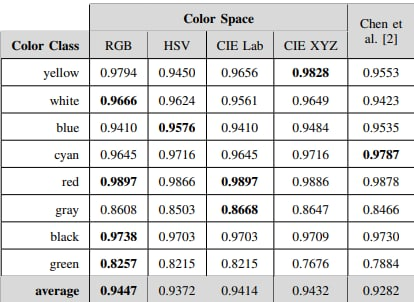
\includegraphics[height=2in, width=2.6in]{Images/table1.jpg}}}
      \caption{Accuracy with 4 color values}
      \label{fig:1}
\end{figure}

\subsection*{\bf HDR (Handwritten Digit Recognition)}
\subsubsection*{\bf Dataset}

MNIST, which comprises of 70,000 handwritten raster pictures from 250 different sources, was the main dataset. I used to train the model. Of these, 60,000 were utilized for training, while the remaining 15,000 were used for training validation. Figure 1 shows how MNIST data are represented in the png file format. Pre-processing, Data Encoding, Model Construction, Training and Validation, Model Evaluation, and Prediction are the main stages of our suggested methodology. All the stages follow the loading of the dataset because it is a prerequisite for all processes. \par

\begin{figure}[thpb]
      \centering
      \framebox{\parbox{2.6in}{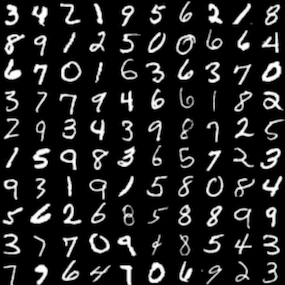
\includegraphics[height=2in, width=2.6in]{Images/mnist.png}}}
      \caption{MNIST Data}
      \label{fig:1}
\end{figure}

We divided the data into X and Y after importing it, where X is the image and Y is the label that goes with it. Convolution serves as the initial layer or input layer for our model. We must rearrange the pictures such that each pixel value is in its own space since convolution treats each pixel as a neuron. This transforms a 28x28 matrix of greyscale values into a 28x28x1 tensor. We may divide the photos into train and test for next stages whether they are all the correct dimensions. \par

The model consists of binary classification and feature extraction using convolution. To extract the features from the picture, convolution and max-pooling are used. On a 28x28 image, 32 3x3 convolution filters are applied, followed by a max-pooling layer with a 2x2 pooling size, and then a second convolution layer with 64 3x3 filters. Finally, we have 7x7 photos that we can flatten. The flatten layer will reduce the 7x7 pictures to a set of 128 values, which will then be mapped to a dense layer of 128 neurons linked to the category output layer of 10 neurons. \par

\section{\bf Experiment result}
\subsection*{\bf HGR (Hand Gesture Recognition)}
I have tried two approaches. The former one: \par 
The DHG dataset is what we use. Every sequence goes through the preprocessing steps outlined in the section before. Each resampled skeleton sequence is broken down into 22 joint sequences, followed by three 1D sequences representing the joint's (x, y, z) coordinates. Thus, the model we developed receives 66 = 22 + 3 input sequences. The labels we will assign to the gesture corresponding to the 66-channel input are represented by the outputs of the last layer of the MLP. We employ two separate neural networks with the same design, but one has 14 outputs and the other has 28, because there are two classification jobs depending on the number of classes. \par

Our model performs well on the DHG dataset, achieving classification accuracy for the 14 gesture classes case of 91.28\% and the 28 gesture classes case of 84.35\%. \par

In classification, precision is defined as the ratio
precision $= \frac{TP}{TP + FP}$ where $TP$ is the number of true positives and $FP$ the number of false positives, while recall is defined as the ratio recall $=\frac{TP}{TP+FN}$ where $TP$ still is the number of true positives and $FN$ is the number of false negatives.

Another approach has better result: our algorithm correctly categorizes various hand gestures photographs with sufficient confidence {\bf >95\%} based on a Deep Learning model based on the findings shown in the previous section. \par

Several features of our challenge have a direct impact on how accurate our model is. The visuals are crisp and background-free, and the motions displayed are rather distinct. Additionally, there are a sufficient number of photos, which strengthens our model. The disadvantage is that we would likely require additional data for various challenges in order to properly influence the parameters of our model. A deep learning model is also particularly challenging to comprehend because of its abstractions. \par
\subsubsection*{\bf Architectural differences}
Branch ablation: There are a ton of other model architectural configurations that might be used, such as weights sharing or progressive channel fusion. Convolution kernel sizes of 3 and 7 were chosen for the current model, for example, due to a partial grid search. With 14 gestures, removing the residual (res. high, low) branch from the model results in a slight accuracy degradation of 1.05\% (resp. 0.53\%, 1.31\%). However, we may emphasize the significance of the three parallel branches since with 28 classes, the model's accuracy drops significantly (by 5.24\% vs. 6.38\% vs. 4.96\%).

\subsection*{\bf VCR (Vehicle Color Recognition)}
Fig. 2 shows that the RGB color space has the highest average accuracy during the testing process, at 94,47\%. The models' four employed color spaces have a high accuracy of more than 90\% and a little variance. The outcomes demonstrate that our CNN model outperforms the original dataset system. In the color categories of yellow, white, blue, red, gray, black, and green, our models outperform. Our system only had a lower accuracy of 0.7\% for the cyan color class. The confusion matrix reveals that the green and gray color classes are where our model performs the lowest in terms of accuracy. Some green class samples are mistakenly labeled as gray class, and this rate is above 10\%. As observed in the dataset, several samples of the green color class contain colors that are quite similar to gray, looking more like greengray than green, hence the classifier could have incorrectly categorized them as belonging to the gray color class. The identical instance may be found in the gray color category, which some gray color class examples mistakenly labeled as the white color category. \par
The network's initial convolutional layer is crucial for extracting low-level characteristics. Layers conv1 and conv2 of our CNN architecture's first convolutional layer and an example output of the pooling process. Rich color characteristics in the input picture are captured by the first convolutional layer. The kernels contain every variation in car color found in the dataset. A lot of cyan-like color is captured by the network 1 kernels. The cyan color class or the red color class may both be influenced by cyan-like colors found in the kernel. \par
The majority of the photos in the dataset being taken from a height with a little angle variation, which leaves the side of the automobile with limited coverage. The camera arrangement used to capture the images in the dataset simulates a CCTV or other street camera that has historically been set up in a similar manner. \par

\subsection*{\bf HDR (Handwritten Digit Recognition)}
We need to perform a small amount of picture pre-processing on the real-world photographs because the model was trained on greyscale raster images. After pre-processing, we use a neural network to predict the label of the picture using the pre-processed image. A list of 10 activation values, ranging from 0 to 9, is the result we receive. The projected label for the image is at the position with the highest value. \par

When our model obtained 99.55\% training accuracy and 99.16\% validation accuracy with a 5\% training loss and 4\% validation loss, it ended training at the second epoch. \par

\begin{figure}[thpb]
      \centering
      \framebox{\parbox{2.6in}{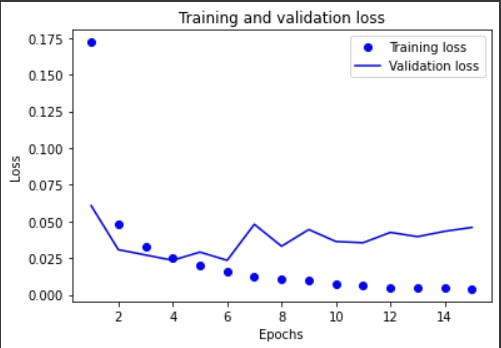
\includegraphics[height=2in, width=2.6in]{Images/gr2.jpg}}}
      \caption{Training and validation loss}
      \label{fig:1}
\end{figure}

\begin{figure}[thpb]
      \centering
      \framebox{\parbox{2.6in}{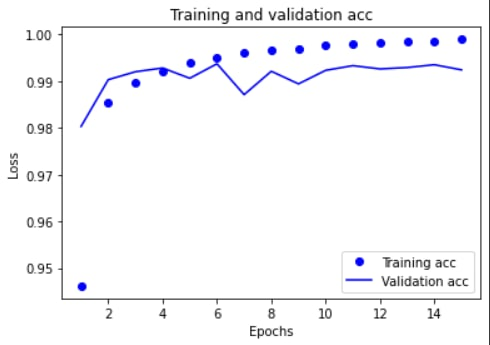
\includegraphics[height=2in, width=2.6in]{Images/gr3.jpg}}}
      \caption{training and validation accuracy}
      \label{fig:1}
\end{figure}

Both handwritten and computer-generated numbers can be recognized by our approach. Compared to real-world digit prediction, computer-generated digit prediction is more precise.

\section{\bf Conclusions}
\subsection*{\bf HGR (Hand Gesture Recognition)}
In this research, we propose a unique key frames extraction approach and feature fusion strategy to construct a quick and reliable gesture detection system. Our novel key frame extraction approach, which is based on picture entropy and density clustering and can significantly minimize the redundant information of the original video, is proposed in consideration of the speed of recognition. Additionally, we provide a powerful feature fusion technique that combines visual and motion signals for reliable hand gesture detection.

\subsection*{\bf VCR (Vehicle Color Recognition)}
In the study, we offer a convolutional neural network-based system for recognizing the color of a car. Our model outperforms Chen's first method and successfully captures vehicle color with a 94,47\% accuracy rate. According to the experiment, utilizing the RGB color system yields the best accuracy, which is in direct opposition to other articles that suggest using the HSV color space instead of the RGB color space for color recognition.

\subsection*{\bf HDR (Handwritten Digit Recognition)}
CNN fared greatly when it came to handwriting recognition. The suggested technique has a 99.5\% accuracy rate and can recognize real-world photos as well; both the training and assessment loss percentages are low at less than 0.1. The noise in the real-world photograph is the sole difficult aspect that needs to be taken care of. The cross-validation measure and the number of dense neurons have a significant impact on the model's learning rate.


\addtolength{\textheight}{-12cm}   % This command serves to balance the column lengths
                                  % on the last page of the document manually. It shortens
                                  % the textheight of the last page by a suitable amount.
                                  % This command does not take effect until the next page
                                  % so it should come on the page before the last. Make
                                  % sure that you do not shorten the textheight too much.

%%%%%%%%%%%%%%%%%%%%%%%%%%%%%%%%%%%%%%%%%%%%%%%%%%%%%%%%%%%%%%%%%%%%%%%%%%%%%%%%
\newpage
\section*{Acknowledgments}

I would like to thank Prof. Uddin Ahmed Minhaz for the course-base and the concern about the project structure and suggestions. The assignments and the materials provided were like "Higgs boson" to create this project paper.


%%%%%%%%%%%%%%%%%%%%%%%%%%%%%%%%%%%%%%%%%%%%%%%%%%%%%%%%%%%%%%%%%%%%%%%%%%%%%%%%


\begin{thebibliography}{99}

\bibitem{c1} Convolutional neural network. (2022, November 16). Wikipedia. \url{https://en.wikipedia.org/wiki/Convolutional\_neural\_network}

\bibitem{c2} Wikipedia contributors. (2022, November 24). Gesture recognition. Wikipedia. \url{https://en.wikipedia.org/wiki/Gesture\_recognition}

\bibitem{c3} Wikipedia contributors. (2022a, November 10). Handwriting recognition. Wikipedia. \url{https://en.wikipedia.org/wiki/Handwriting\_recognition}

\bibitem{c4} Géron, A. (2022). Hands-On Machine Learning with Scikit-Learn, Keras, and TensorFlow: Concepts, Tools, and Techniques to Build Intelligent Systems (3rd ed.). O’Reilly Media.

\bibitem{c5} Russell, S., \& Norvig, P. (2022). Artificial Intelligence: A Modern Approach. Pearson India Education Services Private Limited.

\bibitem{c6} Kapoor, A., Gulli, A., Pal, S., \& Chollet, F. (2022). Deep Learning with TensorFlow and Keras: Build and deploy supervised, unsupervised, deep, and reinforcement learning models, 3rd Edition (3rd ed.). Packt Publishing.

\bibitem{c7} Fast and Robust Dynamic Hand Gesture Recognition via
Key Frames Extraction and Feature Fusion

\bibitem{c8} Reza Fuad Rachmadi, \& I Ketut Eddy Purnama. (2015). Vehicle Color Recognition using Convolutional Neural Network. ArXiv: Computer Vision and Pattern Recognition.

\bibitem{c9} Zhang, Q., Zhuo, L., Li, J., Zhang, J., Zhang, H., \& Li, X. (2018). Vehicle color recognition using Multiple-Layer Feature Representations of lightweight convolutional neural network. Signal Processing, 147, 146–153. \url{https://doi.org/10.1016/j.sigpro.2018.01.021}

\bibitem{c10} Effective Handwritten Digit Recognition using Deep Convolution
Neural Network

\bibitem{c11} Effective Handwritten Digit Recognition using Deep Convolution
Neural Network

\bibitem{c12} He, K., Zhang, X., Ren, S., \& Sun, J. (2015). Delving Deep into Rectifiers: Surpassing Human-Level Performance on ImageNet Classification. 2015 IEEE International Conference on Computer Vision (ICCV). \url{https://doi.org/10.1109/iccv.2015.123}

\bibitem{c13} Tsai, L. W., Hsieh, J. W., \& Fan, K. C. (2007). Vehicle Detection Using Normalized Color and Edge Map. IEEE Transactions on Image Processing, 16(3), 850–864. \url{https://doi.org/10.1109/tip.2007.891147}

\end{thebibliography}

\end{document}